\documentclass[finalversion]{usetex-v1}

%% For intial submission uncomment the following code to remove ednote
%% comments

%\makeatletter{}
%\newsavebox{\kfl@discard}
%\renewenvironment{ednote}[1]{\@latex@warning
%  {Leftover ednote environment in final version ignored}%
%  \begin{lrbox}{\kfl@discard}}{\end{lrbox}}
%\makeatother{}

% In addition, the option "endnotes" permits the use of the
% otherwise-disabled, Usenix-deprecated footnote{} command in
% documents.  In this case, be sure to include a
% \makeendnotes command at the end of your document or
% the endnotes will not actually appear.
%
\usepackage{preamble}


% Hack
\setcounter{secnumdepth}{1}

\begin{document}

\title{mGTK: An \sml binding of \gtk\\\relax[Extended Abstract]}

\docstatus{Submitted to USENIX'04 (FREENIX track)}

\author{
\authname{Ken Friis Larsen}
\authaddr{(Work done while at ITU)}
%\authaddr{Your Institution}
%\authaddr{ Your City, State, ZIP}
\authurl{\url{ken@friislarsen.net}}
%\authurl{\url{http://host.dom/yoururl}}
\and
\authname{Henning Niss}
\authaddr{Department of Innovation}
\authaddr{IT University of Copenhagen}
\authaddr{Denmark}
\authurl{\url{hniss@it.edu}}
%
} % end author

\maketitle

\DefineShortVerb{\!}

\begin{abstract}
  We describe \mgtk a language binding that makes the graphical
  toolkit \gtk, written in C, accessible from programs written in the
  programming language Standard~ML (\sml).  This is not a trivial task
  because \gtk is based on an object-oriented widget hierarchy and
  \sml is a functional language with a non--object-oriented type
  system.  In this paper we describe how it is possible to encode a
  single-inheritance class-hierarchy using \sml's type system and we
  describe how we machine-generate most of the binding to best utilize
  the limited man-power of the project.
\end{abstract}



\section{Introduction}
\label{sec:intr-backgr}

This section gives a brief introduction to \sml and \gtk, and presents
an overview of the rest of the paper.

\textit{[Note to PC: We decided to remove some motivation and background
  in favor of an introduction to \sml; in the final version we expect
  to start out with motivation and background.]}

\begin{ednote}{Ken}
  * Hvad med at motivere og forklare hvorfor vi vil have et grafisk lib
  til SML.

  * SML er ikke OO (tester Gtk+-folkenes "hypotese")
\end{ednote}

\subsection{Standard ML}

\begin{ednote}{Ken}
  Take one.  It is crap but is it here
\end{ednote}

Standard ML (\sml) is a functional language with imperative features
widely used for teaching and in research.  It is roughly on the same
level of abstraction as Python or Scheme. In contrast to Python and
Scheme, which are \emph{dynamically typed}, \sml is \emph{statically
  typed} (like Java and C++) which means that type errors are detected
at \emph{compile time} rather than at \emph{run time}.  Despite \sml
being statically typed, it is not necessary for the programmer to
explicitly provide type annotations in the program, because \sml
features \emph{type inference} which means that the compiler
reconstructs type annotations as needed.
%  \sml also features algebraic
%datatypes, pattern-matching, tuples and records, first-class and
%anonymous functions, exception handling, immutable data types and
%updatable references, abstract data types, and parametric modules, but
%it is outside the scope of this paper to introduce all these features,
%instead we refer the interested reader to one of the fine textbooks
%\cite{Hansen-Rischel:1999,Paulson:1996}.

\begin{ednote}{Ken}
  Skulle vi have et lille fac og fib eksempel?
  (drop for extended abstract)
\end{ednote}

\sml is one of the few languages with a formal definition
\cite{Milner:1997:Definition}.  The definition defines \sml in 93
pages of mathematical notation and English prose.  The book is not
meant as tutorial for the language, its existence is rather to provide
an implementation-independent formulation of \sml.  This formal
definition means that it is possible to write substantial applications
in \sml which are not dependent on a specific compiler, also there
are several mature \sml implementations with widely different
implementation strategies ranging from byte-code interpreters with
interactive \emph{read--eval--print--loops} (REPLs) to aggressively
optimizing whole-program compilers targeting native code.


\begin{ednote}{Ken}
  Introduce modules.  Just signatures and (nested) structures.
  (m�ske drop for extended abstract)
\end{ednote}


\subsection{\gtk}
\label{sec:gtk}

\gtk (GIMP Toolkit) is a library for creating graphical user
interfaces. It is licensed using the LGPL. It is the graphical toolkit
used in the \gnome platform.  \gtk is implemented in C, but from the
beginning the \gtk developers have paid attention to making it feasible
and practical to develop bindings for other programming languages than C.


%\subsection{Overview of this paper}
%\label{sec:overview-this-paper}



\section{Running Example}
\label{sec:example}

Figure~\ref{fig:hello-world} shows a deliberately simple Hello World
example using \mgtk. It illustrates (1) how to get the toolkit
initialized using \texttt{GtkBasis.init} (from a module containing
basic \gtk functionality not related to specific widgets), (2) how to
construct new widgets (using module \texttt{Window} for the Window
widget, and \texttt{Button} for the Button widget), and (3) how to
connect signals to widgets (using module \texttt{Signal}).
\begin{figure*}[htbp]
\begin{centering}
\begin{verbatim}
structure HelloWorld = struct
  fun hello _ = print "Hello World\n"

  fun main _ =
      let val _ = GtkBasis.init(CommandLine.name()::CommandLine.arguments())
          val window = Window.new ()
          val button = Button.new_with_label "Hello World"
      in  Signal.connect window (Widget.delete_event_sig (fn _ => false))
        ; Signal.connect window (Widget.destroy_sig GtkBasis.main_quit)
        ; Signal.connect button (Button.clicked_sig hello)
        ; Container.add window button
        ; Widget.show_all window
        ; GtkBasis.main() 
      end
end

val _ = HelloWorld.main()
\end{verbatim}
\caption{Hello World in \mgtk.\label{fig:hello-world}}
\end{centering}
\end{figure*}

In the figure we use the following \sml constructs (see a textbook on
\sml for further examples; \cite{Hansen-Rischel:1999,Paulson:1996} for
example). All definitions are collected into the module (or
\emph{structure}) \texttt{HelloWorld} whose extent is delimited by
\texttt{struct} \ldots\ \texttt{end}. Informally speaking, a
\emph{signature} is the type of a structure. It specifies the
declarations of the structure that is to be visible from the outside.
The construct \texttt{fun} \textit{foo} \textit{x} \texttt{=}
\textit{exp} declares a function \textit{foo} that has one formal
parameter \textit{x} and function body \textit{exp}; \texttt{fn}
\textit{x} \texttt{=>} \textit{exp} denotes a similar \emph{anonymous}
function. If one does not care about the parameter, one can use the
\emph{wildcard} \texttt{\_}. The construct \texttt{let}~\texttt{val}
\textit{x} \texttt{=} \textit{exp} declares the identifier \textit{x}
to be bound to the value obtained by evaluating \textit{exp}. If the
only reason for evaluating \textit{exp} is any potential side effect,
one can again use the wildcard \texttt{\_}. Expressions evaluated for
their side effects only can also be sequentialized using \texttt{;}.
The value \texttt{()}, ``unit'', can be used as is and is also used as
the return value of purely side-effecting functions.  Finally,
\textit{Foo}\texttt{.}\textit{bar} denotes the value bound to the
identifier \textit{bar} in module \textit{Foo}, and \texttt{::}
denotes the cons operation on lists as in
\textit{hd}\texttt{::}\textit{tl}.

Example base types are {\tUnit} for the unit value \texttt{()},
{\tInt} for integer values, and {\tBool} for boolean values. The type
of a list of integers is \tList{\tInt}. The type of a function
expecting an integer list argument and returning an integer result is
\tArrow{(\tList\tInt)}{\tInt}; the \textit{length} function on lists
would have such a type, for example. 

%% Some functions never need to
%% ``inspect'' (sub)parts of supplied arguments values; such functions
%% are called \emph{polymorphic}. For example, the function that just
%% returns it's argument unchanged (the ``identity function'') is
%% polymorphic; so is the function that computes the length of a list. We
%% indicate the parts of the values that are not inspected by using type
%% variables $\alpha, \beta, \ldots$ at the corresponding locations in
%% the type. For example, the type of the identity function is
%% $\tArrow{\alpha}{\alpha}$ telling us that we can apply it to any type of
%% argument, and we get back a value of the same type. The
%% \textit{length} function has type $\tArrow{\tList\alpha}{\tInt}$
%% because, regardless of the type of elements in the list (here denoted
%% $\alpha$), the function can compute the length of the list. Such type
%% variables are \emph{instantiated} to (more) specific types when we
%% apply the polymorphic function. For example, when we apply the
%% polymorphic identity function to \texttt{()} we instantiate $\alpha$
%% to {\tUnit} giving this occurrence of the function the type
%% \tArrow\tUnit\tUnit; when we apply it to \texttt{17} we instantiate
%% $\alpha$ to {\tInt} and the occurrence of the function gets type
%% \tArrow\tInt\tInt. The function is said to be (parametric) polymorphic
%% because we can apply it to arguments of many shapes.

Some functions never need to
``inspect'' (sub)parts of supplied arguments values; such functions
are called \emph{parametric polymorphic}. For example, the 
function \textit{length} that computes the length of a list is polymorphic. We
indicate the parts of the values that are not inspected by using type
variables $\alpha, \beta, \ldots$ at the corresponding locations in
the type. Then the type of \textit{length} is
 $\tArrow{\tList\alpha}{\tInt}$
because, regardless of the type of elements in the list (here denoted
by $\alpha$), the function can compute the length of the list. Such type
variables are \emph{instantiated} to (more) specific types when we
apply the polymorphic function. For \textit{length}, when we
apply it to a list of booleans we instantiate $\alpha$
to {\tBool} giving this occurrence of the function the type
\tArrow{\tList\tBool}\tInt; when we apply it to a list of
integers  we similarly instantiate
$\alpha$ to {\tInt}.

\section{Encoding of classes}
\label{sec:encoding-classes}

As described in Section~\ref{sec:intr-backgr}, \sml in is a functional
language without object-oriented features and \gtk is designed as an
object-oriented library.  Thus, it is not trivially clear how to make an \sml
interface to \gtk.  The most difficult problem is how to present the
subtype relations defined by a class hierarchy in \sml's type system.
That is, in this section we are only interested in how to present a
type-safe \sml interface to \gtk class hierarchy.  By \emph{type-safe} we
mean that, if an \sml application programmer uses our library and
makes a type-error when using the \gtk library, calling a undefined
method on object, for instance, then the \sml compiler should give an
type error (at compile-time).

Fortunately, we are able to take advantage of two properties of \gtk
and \sml.  First, \gtk implements a class system with only
single-inheritance.  Second, \sml's type system is expressive enough
to express the subtype-relations of single-inheritance class
hierarchies.

In type theoretical jargon, the trick is to use \emph{parametric
  polymorphism} and \emph{existential types} to encode inheritance
subtyping.  In particular we use \emph{phantom types} to encode the
inheritance path.


\begin{figure}
  \centering
 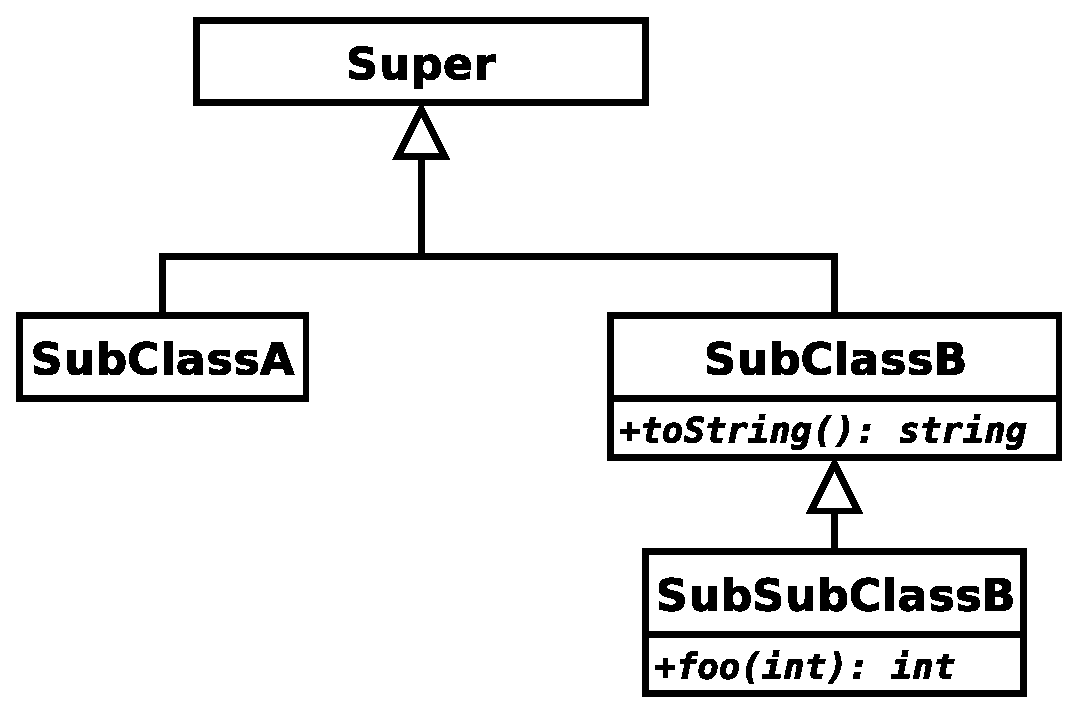
\includegraphics[width=\linewidth]{example-class-diagram.eps}
  \caption{Small example class hierarchy}
  \label{fig:class-hierarchy}
\end{figure}

Figure~\ref{fig:class-hierarchy} shows a small class hierarchy with
four classes; \classname{SubClassA} and \classname{SubClassB}
are subclasses of the class \classname{Super} and
\classname{SubSubClassB} is a subclass of \classname{SubClassB}.  We
shall go through the different parts of the encoding of a class.

\medskip
\noindent\textbf{Class types}\qquad A base class like \classname{Super} in
  Figure~\ref{fig:class-hierarchy} is encoded as an abstract
  parameterized type:
\begin{SMLcode}
type 'path super
\end{SMLcode}
(we follow the \sml convention and spell type-names in lower-case with
underscores if needed).  The type variable !'path! will be used to
hold the inheritance path for subclasses.

\medskip
\noindent\textbf{Subtyping/Inheritance}\qquad For a subclass like \classname{SubClassA}
  we need to declare two new \sml types: an abstract parameterized
  type, which we shall call a \emph{witness type}; and a type
  abbreviation specifying the inheritance:
\begin{SMLcode}
type 'path sub_class_a_t
type 'path sub_class_a = 
        'path sub_class_a_t super
\end{SMLcode}
where !sub_class_a_t! is the witness type and !sub_class_a! is the
type specifying the inheritance.  In the declaration of !sub_class_a!
we see that the type variable !'path! in the declaration of the type
!super! has been instantiated with the type expression 
!'path sub_class_a_t!, which contains an new type variable (also named
!'path!).

In the rest of the paper we shall use the convention that witness
types ends with !_t!.

\medskip
\noindent\textbf{Methods}\qquad Because \sml is not an object-oriented language we shall
  model methods with ordinary functions, and use the usual convention
  that the first argument is the object on which the method is called
  (\gtk also uses this convention).
  
  We can now write the type for the method !toString! in
  \classname{SubclassB}:
\begin{SMLcode}
val toString : 'path sub_class_b 
                             -> string
\end{SMLcode}
This type says that !toString! takes any object which is a subclass of
\classname{SubClassB} and returns a string as result.   Similar the
type for the method !foo! from class \classname{SubSubClassB} has the
type:
\begin{SMLcode}
val foo : 'path sub_sub_class_b 
                         -> int -> int
\end{SMLcode}
That is, !foo! takes any object which is a subclass of
\classname{SubSubClassB} and an integer and returns an integer.

\medskip
\noindent\textbf{Constructors}\qquad We have to be a bit careful with constructors.  If
  we were to return a value with a polymorphic type-variable !'path!
  that holds an inheritance path that has not yet been ``plugged'',
  then we can accidently use a super-class constructor to construct
  values that can be instantiated to the type of a sub-class.  Hence,
  we introduce the abstract dummy type !base! and use that to plug the
  type variable.  Thus, the type of the constructor for
  \classname{SubClassA} is:
\begin{SMLcode}
val new : unit -> base sub_class_a
\end{SMLcode}
The convention in \gtk is that constructors are named !new!.

Then we wrap all parts of an encoding of a class into a structure of
its own.  That is, for the class \classname{SubClassB} in
Figure~\ref{fig:class-hierarchy} the \sml signatures is:
\begin{SMLcode}
  signature SubClassB =
  sig
    type 'path sub_class_b_t
    type 'path sub_class_b = 
           'path sub_class_b_t Super.super
    val new : unit 
              -> GtkBasis.base sub_class_b 
    val toString : 'path sub_class_b 
                                 -> string
  end
\end{SMLcode}
We see that this signature relies on two other structures:  The
structure !Super! for the class \classname{Super} and !GtkBasis! for
the dummy class !base!.

Continuing our running example from Section~\ref{sec:example},
the widgets \texttt{window} and \texttt{button} get the following
types
\begin{SMLcode}
val window : 
       base window_t container_t widget_t t
val button : 
       base button_t container_t widget_t t
\end{SMLcode}
(where !t! is represents the top of the hierarchy e.g. Widget, and all
structure prefixes have been omitted).  The types tell us, reading from
left to right, that \texttt{window} is a Window widget that extends
the Container widget, which in turn extends the Widget widget;
similarly for \texttt{button}. They also tell us that \texttt{window}
and \texttt{button} have a common ancestor, namely the Container
widget.  In particular, therefore, we can use both the window and the
button in all contexts expecting a Container.

For example, the function \texttt{Container.add} has type
\begin{SMLcode}
val add : 'path1 container_t widget_t t
             -> 'path2 widget_t t -> unit
\end{SMLcode}
from which we conclude that \texttt{Container.add} expects two arguments:
one which has to be a sub-widget of Container, and one which has to be
a sub-widget of Widget; the function returns the unit value. Considering
the types of \texttt{window} and \texttt{button} above, we see that
the application
%
``!Container.add window button!''
%
is well-typed because \texttt{window} is indeed a sub-widget of 
Container, and \texttt{button} is indeed a sub-widget of Widget.

Consider now another function that only works on Buttons, \texttt{Button.set\_label}, with type
\begin{SMLcode}
val set_label :
    'path button_t container_t widget_t t
                        -> string -> unit
\end{SMLcode}
Thus \texttt{Button.set\_label} expects a sub-widget of Button and a string and returns unit.
If we were to apply this function to the \texttt{window} widget as in
%
``!Button.set_label window!'',
%
we would get a (compile-time) type error saying (essentially) that
a Window widget is not a subclass of a Button widget because the
inheritance paths do not match. Here is the concrete message output
by the Moscow ML compiler
\begin{verbatim}
- Button.set_label window "New label";
! Toplevel input:
! Button.set_label window "New label";
!                  ^^^^^^
! Type clash: expression of type
!   base window_t container_t widget_t t
! cannot have type
!   'a button_t container_t widget_t t
\end{verbatim}

\begin{ednote}{Ken}
  Explain the cool signal thing.
  (drop for extended abstract)
\end{ednote}

\begin{ednote}{Ken}
  How about the implementation of the binding with finalizers and all?
\end{ednote}


\section{Process}
\label{sec:process}

\begin{ednote}{Henning}
  Fra mini muck-up til fuld toolkit
\end{ednote}

\begin{ednote}{Henning}
  What is a binding?
\end{ednote}

In constructing the \mgtk binding we leverage the foresightedness of
the \gtk developers. Early on it was recognized that it would be
important to have a machine-readable ``specification'' of the toolkit.
Essentially the specification would specify the widget classes, the
inheritance hierarchy, and methods and functions in the toolkit. The
specification became known as the \texttt{gtk.defs} file. One could
argue that it is simple enough to extract the same information from
the C header files; however, that incurs an initial hurdle in the
form of a suitable parser that is not present with the easily parsable
defs-format.

\begin{ednote}{Henning} This is crap, but it is there. \end{ednote}

The bulk of the \mgtk binding is constructed automatically from the
\texttt{gtk.defs} file. Based on this automatic construction the
complete binding process is naturally divided in two phases: (1)
binding ``design'', and (2) binding construction. It is important to
note here that the design phase can be carried out for a very small
subset of the complete toolkit after which the construction phase
``mimics'' that for the complete toolkit.
% We refer to the design as a
%\emph{muck-up} and the result as \minimgtk.
This phase separation makes it easier to get the design right simply
because there are fewer issues to deal with, and it makes the work
involved in moving the binding to other \sml compilers manageable
(essentially just ask the compiler writers to provide the equivalent
of the small subset for their compiler; and mimic that during the
construction phase). Of course it also helps when new releases of \gtk are
produced. Most of the work in constructing the binding for the new
release is over when the design for the small subset has been completed.

Let us return to our running example, and look at some example
specifications of widgets, functions, and signals. Figure~\ref{fig:gtk-defs}
shows three entries in the \texttt{gtk.defs} file.
\begin{figure}[htbp]
\begin{centering}
\begin{verbatim}
(define-object Button
  (in-module "Gtk")
  (parent "GtkBin")
  (c-name "GtkButton")
  (gtype-id "GTK_TYPE_BUTTON")
)
(define-function gtk_button_new_with_label
  (c-name "gtk_button_new_with_label")
  (return-type "GtkWidget*")
  (parameters
    '("const-gchar*" "label")
  )
)
(define-signal clicked
  (of-object "GtkButton")
  (return-type "void")
  (when "first")
)
\end{verbatim}
\caption{\texttt{gtk.defs} excerpt.\label{fig:gtk-defs}}
\end{centering}
\end{figure}
The first entry shows the shape of widget specification (defining
\texttt{Button} to be a sub-widget of \texttt{Bin}). The next entry
shows a function specification (that actually is constructor for the
\texttt{Button} widget) with return type \texttt{GtkWidget*} (in the C
implementation) and a string argument. Finally, we show a specification
of a signal on buttons.

%\subsection{Stubs and code generation}
%\label{sec:stubs-code-gener}


%% \section{Synergy}
%% \label{sec:synergy}

%% \begin{ednote}{Henning}
%%   SML + Gtk+ er godt
%%   (drop for extended abstract?)
%% \end{ednote}



%% \section{Supported \sml compilers}
%% \label{sec:supp-sml-comp}

%% \begin{ednote}{Henning}
%%   MLton og Moscow ML (SML.NET med Gtk\#?)
%% \end{ednote}

\section{The \mgtk binding}
\label{sec:mgtk-binding}

The \mgtk binding is available at SourceForge \texttt{http://mgtk.sf.net/}
and is released under the GNU Lesser General Public License
(LGPL).

\textit{[Note to PC: The binding currently available at the above URL
  is for a previous version of \mgtk and \gtk. The version described here is
  being worked upon and will be available soon after January 1.]}

A key aspect of a binding for \sml is the existence of a variety of
compilers (see the reason in Section~\ref{sec:intr-backgr}). This sets
this work apart from other bindings for languages such as Python where
there is only one compiler/system to target. The process as described
above (Section~\ref{sec:process}) allows us to extend the
applicability of the binding to this multitude of \sml
implementations. Combining this with the multitude of platforms for
which one finds \sml and \gtk implementations, gives the application
programmer a unique opportunity to target a large set of platforms
with a single program. The \mgtk binding already targets two of the
main \sml systems, namely \mosml~\cite{Mosml-webpage:2003} and
\mlton~\cite{MLton-webpage:2003}. The authors are currently
looking into the prospects of constructing the binding for other
\sml compilers (in particular, the
\emph{ML Kit with Regions} \cite{MLKit-webpage:2003} and
\emph{SML.NET} \cite{SML.NET-webpage:2003} with \gtksharp).

This potential for compiler independence sets the present
binding apart from other \gtk bindings for \sml (notably, the
\texttt{SML-Gtk} binding for the \sml of New Jersey \sml compiler;
\cite{SML-Gtk-webpage:2003}).


\section{Related work}
\label{sec:related-work}

The list of language bindings for \gtk shows a plethora of different
languages from which \gtk is accessible. In this section we briefly
discuss the bindings most related to \mgtk.

There are two major alternatives for ML-like languages to the \mgtk
binding. (1) The !SML-Gtk! binding mentioned above.
% \url{http://www.cs.nyu.edu/phd_students/leunga/sml-gtk/sml-gtk.html}
%This binding is different from \mgtk in that it is made the ml-nlffi
%bindings generator \cite{Blume:2001:nlffi}, which is currently
%specific to the SML/NJ compiler.  
This binding is specific to the \smlnj compiler (due to its use of
!ml-nlffi!), and also does not handle
memory management. (2) !lablgtk! is a \gtk binding for O'Caml.
% \url{http://wwwfun.kurims.kyoto-u.ac.jp/soft/olabl/lablgtk.html}
O'Caml is a ML dialect different from \sml which (among other things)
has object-oriented features. This binding, therefore, does not have
to \emph{encode} the \gtk object hierarchy.

\gtk has also been bound to other functional languages;
!gtk+hs! is a Haskell binding for example,
% \url{http://www.cse.unsw.edu.au/~chak/haskell/gtk}
and !erlgtk! is an Erlang binding.
% \url{http://erlgtk.sourceforge.net}
%
For \sml, there is also a binding of the Tk toolkit called
!sml_tk!.
% \url{http://www.informatik.uni-bremen.de/~cxl/sml_tk}

The use of phantom types to express invariants about the program
is not new; the encoding of a single-inheritance hierarchy as
above is. Independent work has established similar results
\cite{Fluet-Pucella:2002}. %
On the construction side of things, other bindings are also machine
generated; for this some of the bindings use SWIG, others extract
appropriate information from the C headers files of \gtk.

From the outset the necessity of access to libraries has been realized
in the functional programming community. Work in this area for \sml
include \mosml's C-library support \cite{Larsen:2001} and 
\smlnj's foreign function interface \cite{Blume:2001:nlffi};
for Haskell it includes \cite{Finne:1999:CallingHellFromHeaven}.



\section{Conclusion}
\label{sec:conclusion}

\subsection{Contributions}

In this paper we have demonstrated that it is theoretically and
practically possible to make an interface from \sml to \gtk.  This is
interesting for several reasons: first, the \sml community gets
access to a graphical library which is sourly needed; second, the fact
that it is possible to make an \sml binding to \gtk really attests to
the claimed ``interfaceability'' of \gtk because \sml is so radically
different from C in abstraction level and paradigm; finally, we think
that we have demonstrated that it is indeed possible to bind the entire \gnome
development platform, using mainly machine generated stub code.


\subsection{Future Work}

It is our intention to continue this work by utilizing appropriate
programming language technology to gradually bind more and more of the
\gnome development platform for \sml. As was the case above, this
entails designing appropriate representations of the platform in the
\sml world (in particular as regards the type-safety property mentioned
above) together with the more practical work of extending the code
generator to handle such newly introduced representations.


\bibliographystyle{abbrvnat}
\bibliography{mgtk}

\end{document}

%%% Local Variables: 
%%% mode: latex
%%% TeX-master: t
%%% End: 

% LocalWords:  mGTK FREENIX Friis Niss GtkBasis fn wildcard tl gtk defs SML
% LocalWords:  GtkWidget MLton mgtk
